%prescription_latex.tex

\documentclass{article}
\usepackage[utf8]{inputenc}
\usepackage[spanish]{babel}
\usepackage[T1]{fontenc}
\usepackage{textcomp}
\usepackage{graphicx}
\usepackage{eso-pic}
\usepackage{ifthen}
\usepackage[abs]{overpic}
\usepackage{pict2e,xcolor,varwidth}
\usepackage{color}
\usepackage{layout}
%\usepackage{tikz}
%\usepackage{relsize}
\usepackage{etoolbox}
\usepackage[paperwidth=27.94cm, paperheight=21.59cm, left=0.0cm,right=0.0cm,top=0.0in,bottom=0.0in,headheight=0in,headsep=0pt,footskip=120pt]{geometry}
% Check parameters in: https://en.wikibooks.org/wiki/LaTeX/Page_Layout
%
\graphicspath{ {/vagrant/ersteops/static/img/printpdf/} }
%\setmainfont{Arial}
%\usepackage{fancyhdr}
\usepackage{uarial}
%\usepackage[scaled]{uarial}
\usepackage{transparent}
\usepackage[protrusion=true,expansion=true]{microtype}
\usepackage{calc}
\usepackage{verbatim}
\makeatletter
\g@addto@macro\@verbatim\small
\makeatother 
\usepackage{xcolor}

\usepackage{lmodern}
%\fontfamily{lmss}\selectfont


\begin{document}
\fontfamily{lmss}\selectfont
    % Include Background in ./prescript/media/media/template_v1.pdf
    % \AddToShipoutPictureBG{\ifthenelse{\isodd{\value{page}}}{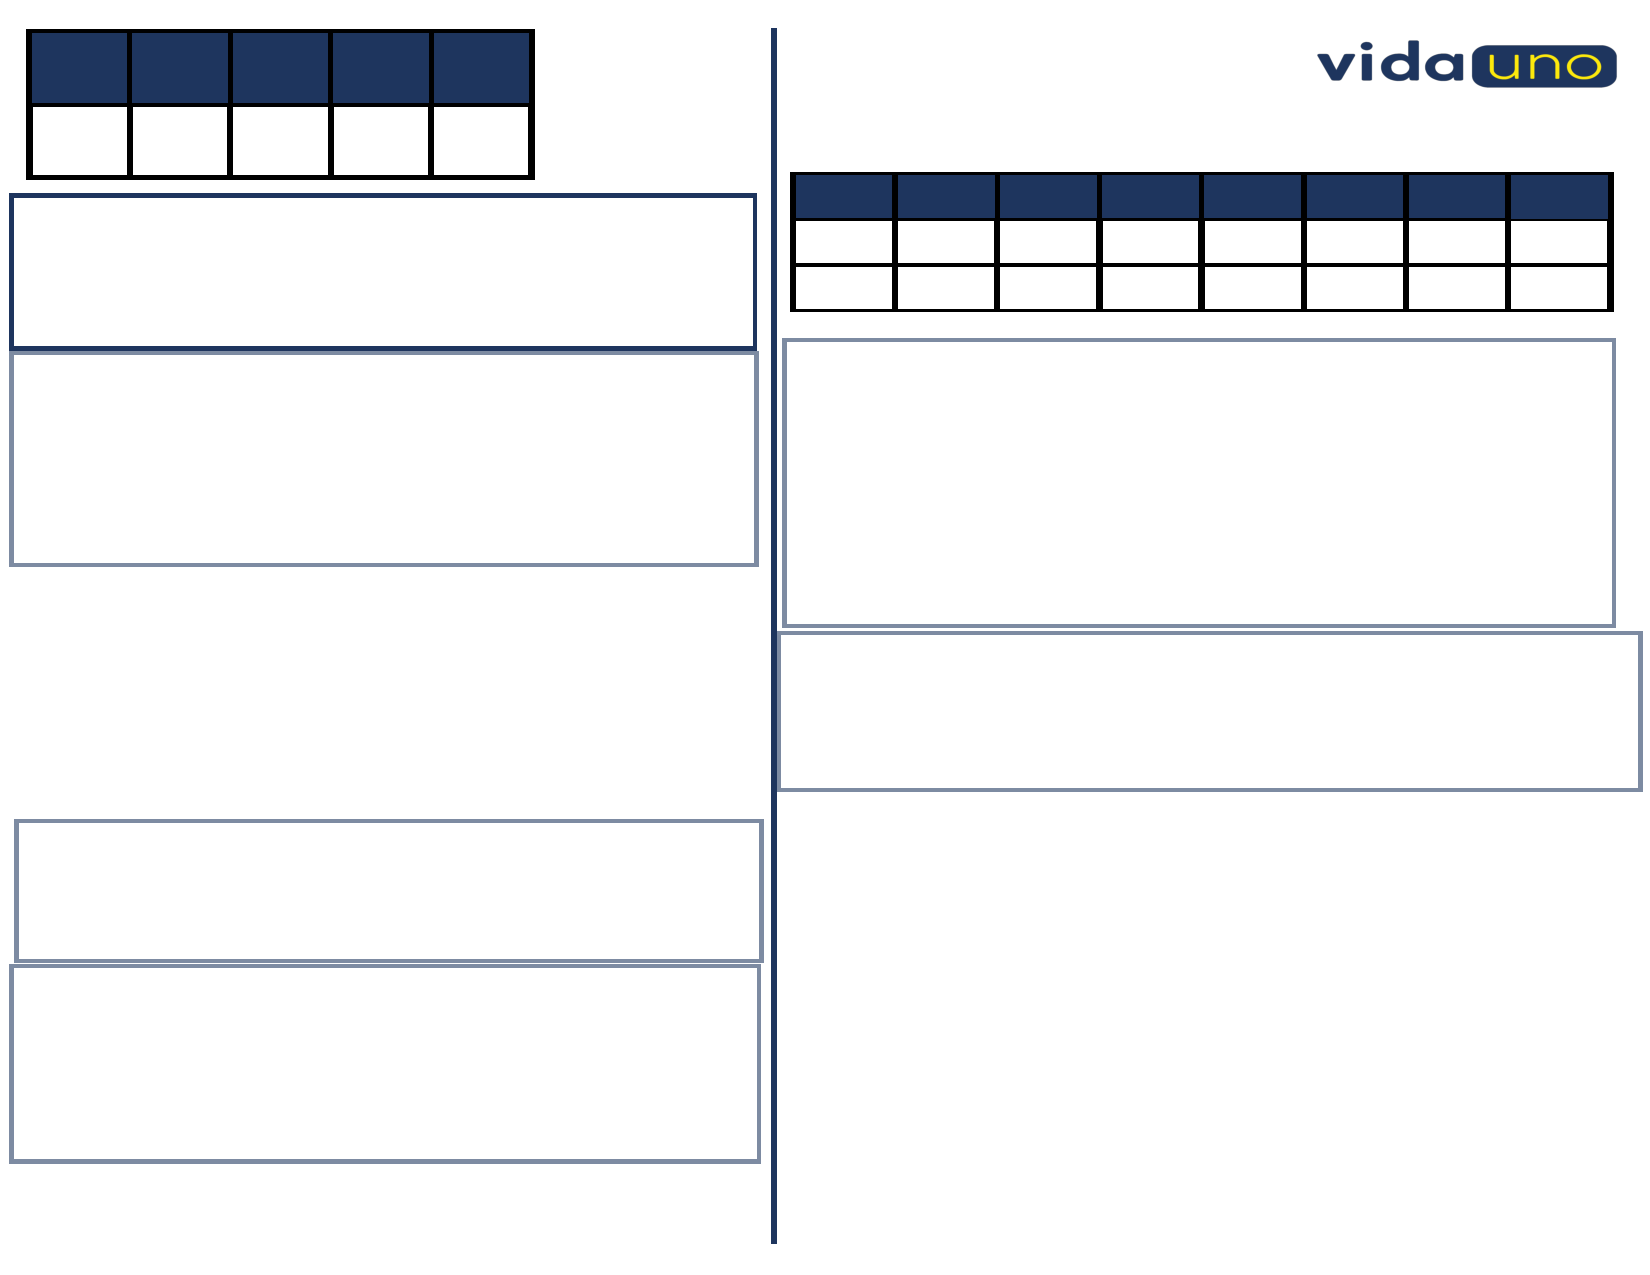
\includegraphics{laam_template}}{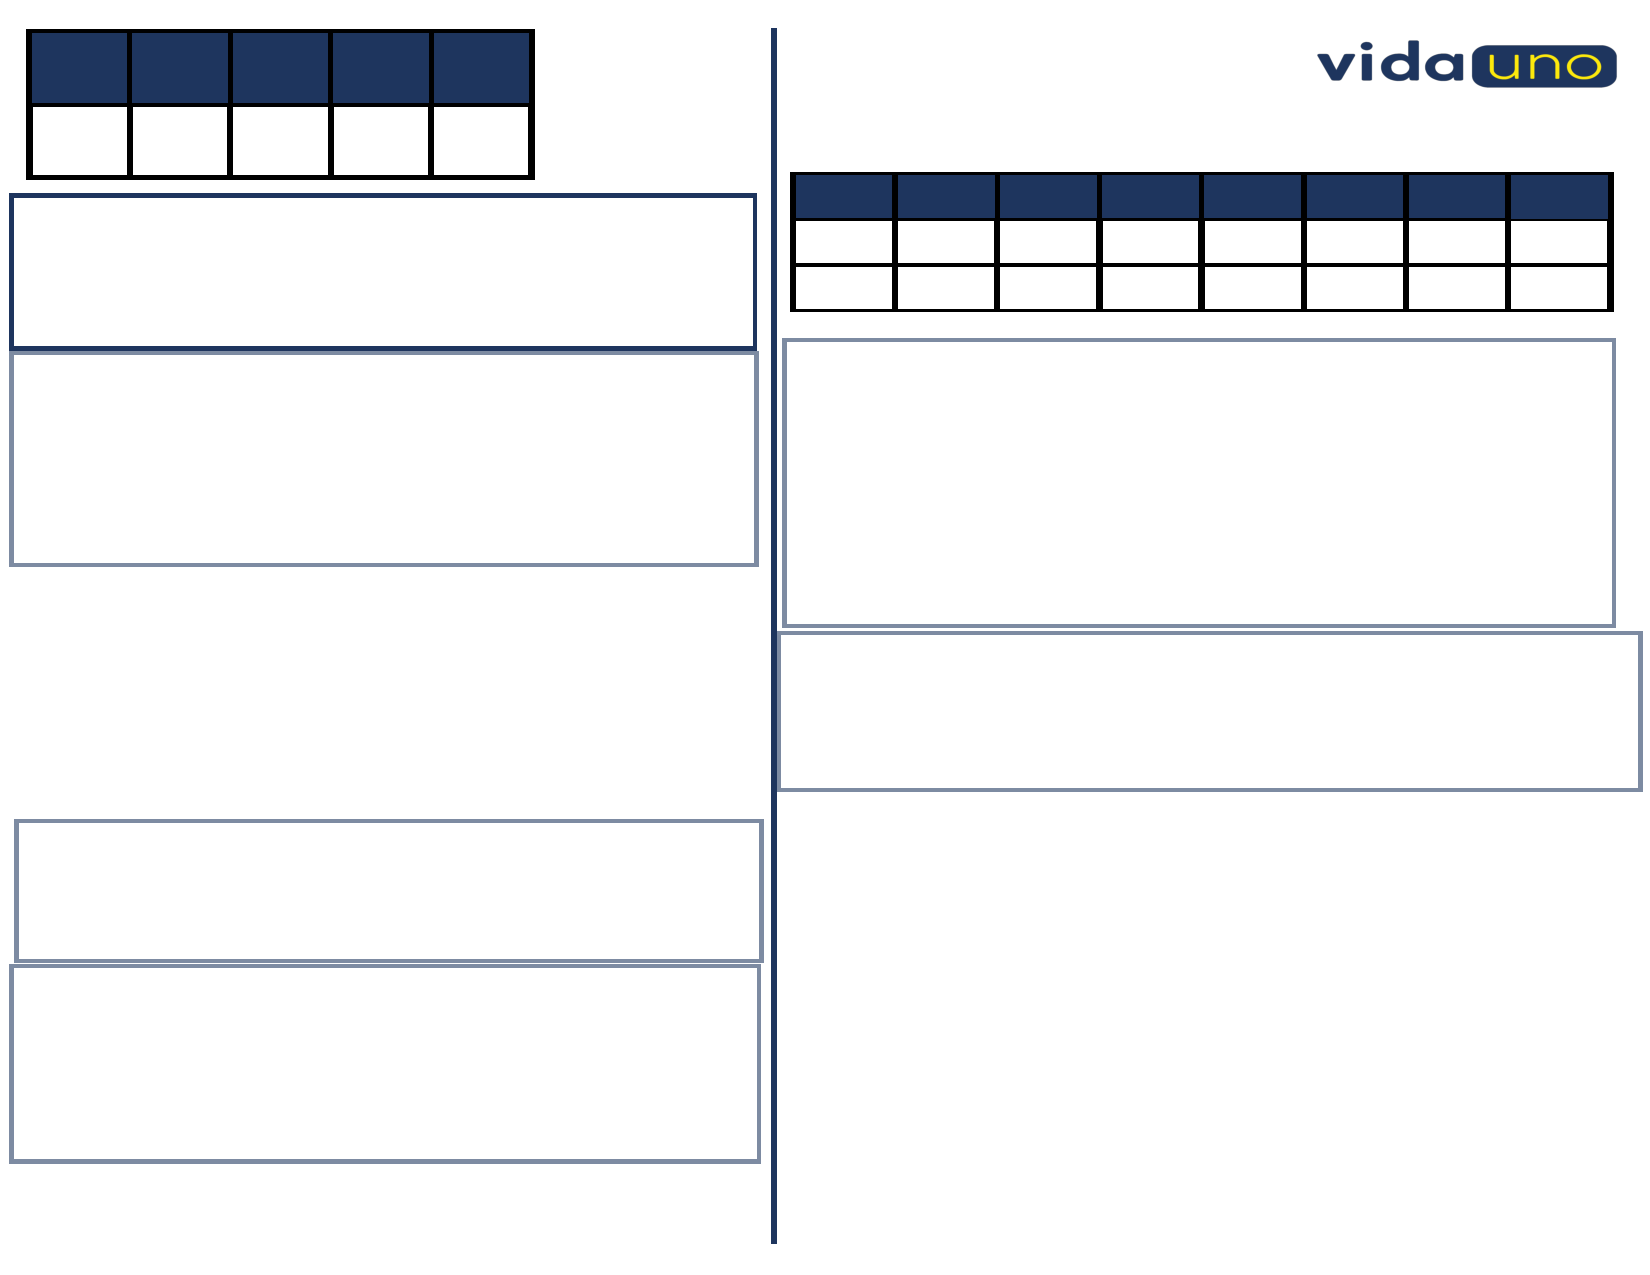
\includegraphics{laam_template}}}
    % Define page content
    %\textsf{\large{
    %\begin{changemargin}{1.5cm}{1.2cm}
        %\begin{enumerate}
            %
            %bla!
        %\end{enumerate}
    %         \put(1,1){\parbox[t]{3cm}{\textsf{\large{
    %    \textbf{Consulta \#:} 16
    % }
    % }}}
        % Indicaciones Extra
        % \begin{enumerate}
        %     \textbf{Indicaciones Extra: \\ } 
        % \end{enumerate}
    %\end{changemargin}
    %}}
    % \begin{picture}(1,0.77272727)%
    %     %Consulta    
    % \put(200,0){\parbox[t]{3cm}{\textsf{\large{
    %    \textbf16
    % }
    % }}}
    % \end{picture}
% \begingroup%
%   \makeatletter%
%   \providecommand\color[2][]{%
%     \errmessage{(Inkscape) Color is used for the text in Inkscape, but the package 'color.sty' is not loaded}%
%     \renewcommand\color[2][]{}%
%   }%
%   \providecommand\transparent[1]{%
%     \errmessage{(Inkscape) Transparency is used (non-zero) for the text in Inkscape, but the package 'transparent.sty' is not loaded}%
%     \renewcommand\transparent[1]{}%
%   }%
%   \providecommand\rotatebox[2]{#2}%
%   \newcommand\scaleInNode[1][1]{\tikzset{execute at begin node={\normalsize\larger[#1]}}}
%   \newcommand*\fsize{\dimexpr\f@size pt\relax}%
%   \newcommand*\lineheight[1]{\fontsize{\fsize}{#1\fsize}\selectfont}%
%   \ifx\svgwidth\undefined%
%     \setlength{\unitlength}{792bp}%
%     \ifx\svgscale\undefined%
%       \relax%
%     \else%
%       \setlength{\unitlength}{\unitlength * \real{\svgscale}}%
%     \fi%
%   \else%
%     \setlength{\unitlength}{\svgwidth}%
%   \fi%
%   \global\let\svgwidth\undefined%
%   \global\let\svgscale\undefined%
%   \makeatother%
%   \begin{picture}(1,0.77272727)%
%     \lineheight{1}%
%     \setlength\tabcolsep{0pt}%
%     \put(0,0){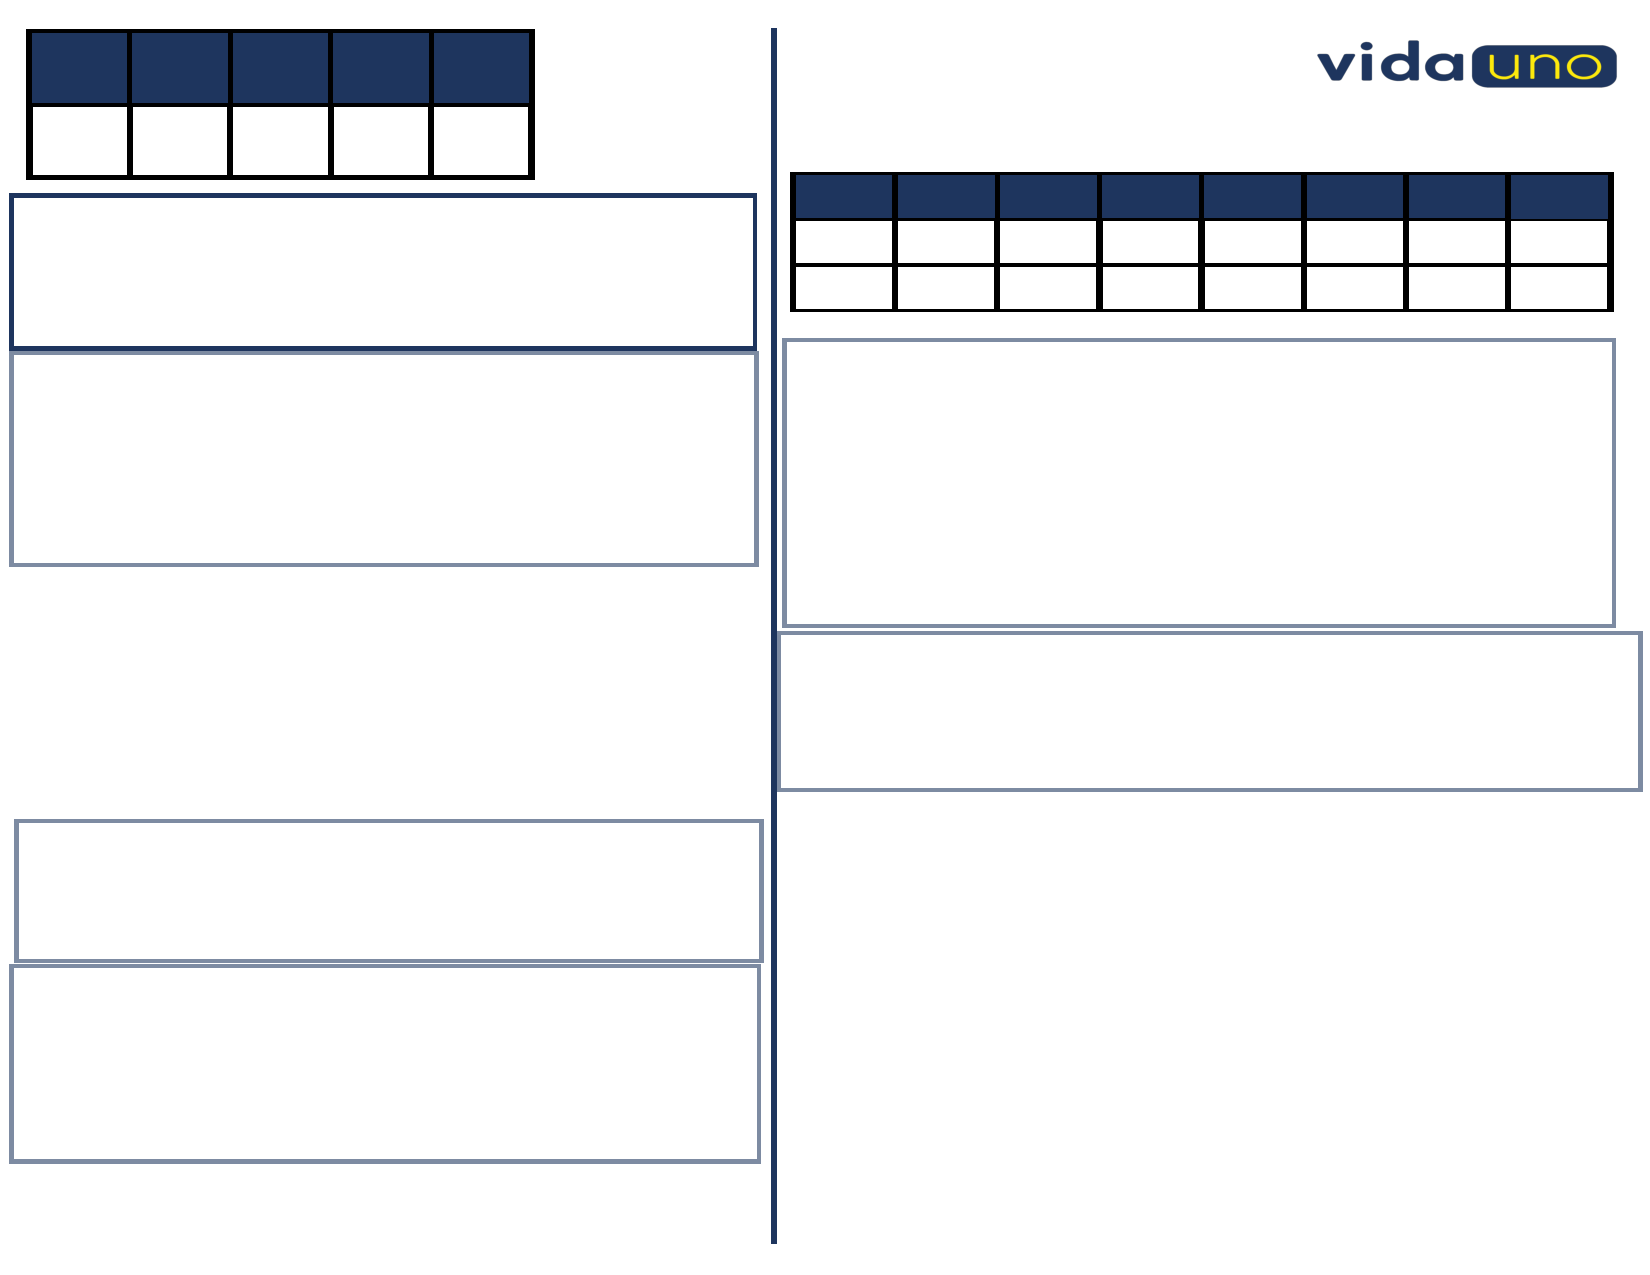
\includegraphics[width=\unitlength,page=1]{laam_template}}%

%     % \put(0.01140896,0.54355203){\parbox[t]{3cm}{\textsf{\large{
%     %    \textbf{Consulta \#:} 16
%     % }
%     % }}}
%     % \put(0.01140896,0.54355203){\color[rgb]{0.11764706,0.20784314,0.36862745}\makebox(0,0)[lt]{\lineheight{1.25}\smash{\begin{tabular}[t]{l}\textbf{Paciente desconocido 16 }\end{tabular}}}}%
% 	\put(0.42718184,0.73912713){\color[rgb]{0,0,0}\makebox(0,0)[lt]{\lineheight{1.25}\smash{\begin{tabular}[t]{l}\textit{ 16 }\end{tabular}}}}%
%    	\put(0.42718184,0.72336542){\color[rgb]{0,0,0}\makebox(0,0)[lt]{\lineheight{1.25}\smash{\begin{tabular}[t]{l}\textit{ M011 }\end{tabular}}}}%
%     \put(0.3690564,0.69389968){\color[rgb]{0,0,0}\makebox(0,0)[lt]{\lineheight{1.25}\smash{\begin{tabular}[t]{l}\textit{ NA }\end{tabular}}}}%
%     \put(0.39254546,0.6775768){\color[rgb]{0,0,0}\makebox(0,0)[lt]{\lineheight{1.25}\smash{\begin{tabular}[t]{l}\textit{ NA }\end{tabular}}}}%

%   \end{picture}%
% \endgroup%

\begin{figure}
  \centering
  \def\svgwidth{\columnwidth}
  %\input{paperless_template_6.pdf_tex}

\begingroup%
  \makeatletter%
  \providecommand\color[2][]{%
    \errmessage{(Inkscape) Color is used for the text in Inkscape, but the package 'color.sty' is not loaded}%
    \renewcommand\color[2][]{}%
  }%
  \providecommand\transparent[1]{%
    \errmessage{(Inkscape) Transparency is used (non-zero) for the text in Inkscape, but the package 'transparent.sty' is not loaded}%
    \renewcommand\transparent[1]{}%
  }%
  \providecommand\rotatebox[2]{#2}%
  \newcommand*\fsize{\dimexpr\f@size pt\relax}%
  \newcommand*\lineheight[1]{\fontsize{\fsize}{#1\fsize}\selectfont}%
  \ifx\svgwidth\undefined%
    \setlength{\unitlength}{782.27360219bp}%
    \ifx\svgscale\undefined%
      \relax%
    \else%
      \setlength{\unitlength}{\unitlength * \real{\svgscale}}%
    \fi%
  \else%
    \setlength{\unitlength}{\svgwidth}%
  \fi%
  \global\let\svgwidth\undefined%
  \global\let\svgscale\undefined%
  \makeatother%
  \begin{picture}(1,0.77245213)%
    \lineheight{1}%
    \setlength\tabcolsep{0pt}%
    \put(0,0){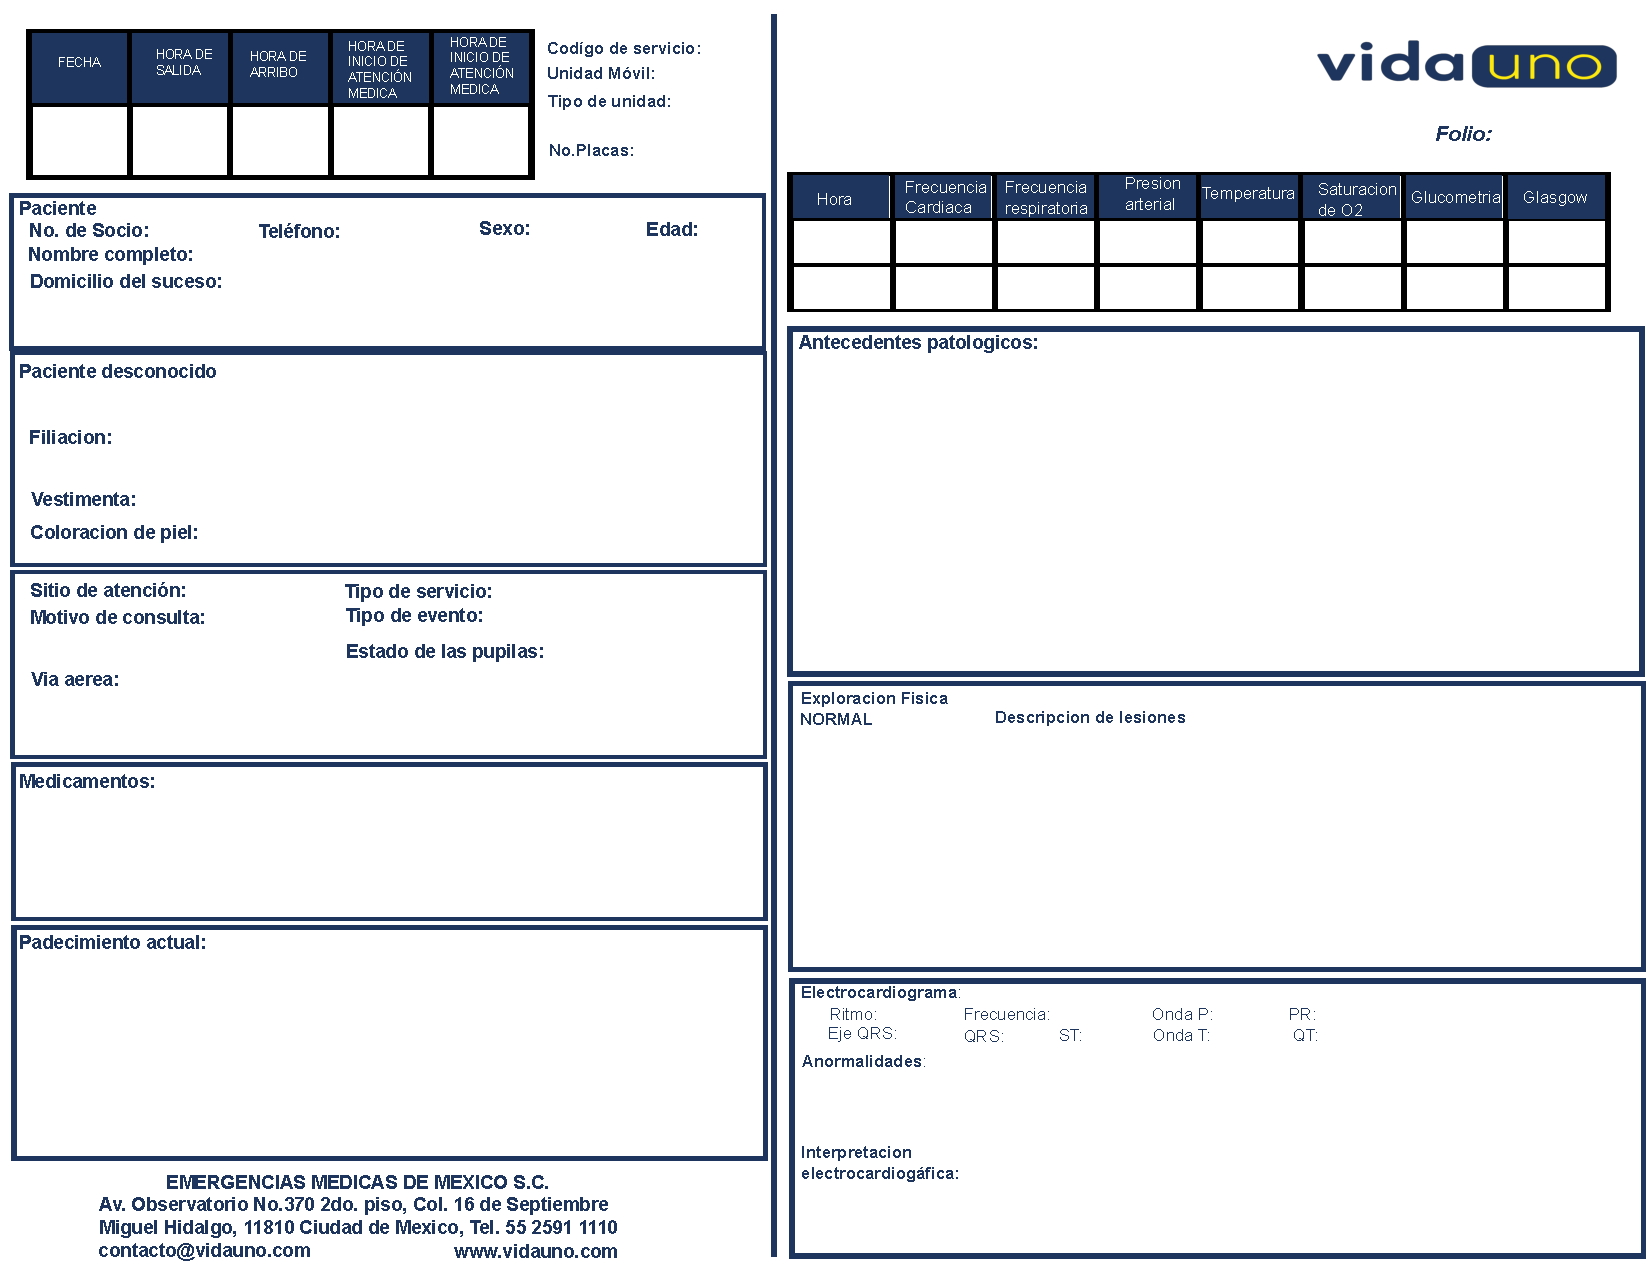
\includegraphics[width=\unitlength,page=1]{paperless_template_page_1}}%

    \put(0.42638971,0.73960084){\color[rgb]{0,0,0}\makebox(0,0)[lt]{\lineheight{1.25}\smash{\begin{tabular}[t]{l}\fontfamily{lmss}\selectfont 11\end{tabular}}}}%
    \put(0.43014479,0.72364315){\color[rgb]{0,0,0}\makebox(0,0)[lt]{\lineheight{1.25}\smash{\begin{tabular}[t]{l}\fontfamily{lmss}\selectfont M011\end{tabular}}}}%
   	\put(0.33829987,0.69381105){\color[rgb]{0,0,0}\makebox(0,0)[lt]{\lineheight{1.25}\smash{\begin{tabular}[t]{l}\fontfamily{lmss}\selectfont NA\end{tabular}}}}%
    \put(0.39132267,0.67728521){\color[rgb]{0,0,0}\makebox(0,0)[lt]{\lineheight{1.25}\smash{\begin{tabular}[t]{l}\fontfamily{lmss}\selectfont NA\end{tabular}}}}%

    %Paciente
    \put(0.09655761,0.62796396){\color[rgb]{0,0,0}\makebox(0,0)[lt]{\lineheight{1.25}\smash{\begin{tabular}[t]{l}\fontfamily{lmss}\selectfont F55\end{tabular}}}}%
    \put(0.20912356,0.62853648){\color[rgb]{0.11764706,0.20784314,0.36862745}\makebox(0,0)[lt]{\lineheight{1.25}\smash{\begin{tabular}[t]{l}\fontfamily{lmss}\selectfont 5556782349\end{tabular}}}}%
    \put(0.3268484,0.62911649){\color[rgb]{0,0,0}\makebox(0,0)[lt]{\lineheight{1.25}\smash{\begin{tabular}[t]{l}\fontfamily{lmss}\selectfont Masculino\end{tabular}}}}%
    \put(0.42764439,0.62796396){\color[rgb]{0,0,0}\makebox(0,0)[lt]{\lineheight{1.25}\smash{\begin{tabular}[t]{l}\fontfamily{lmss}\selectfont 15\end{tabular}}}}%
    \put(0.12766308,0.61324599){\color[rgb]{0,0,0}\makebox(0,0)[lt]{\lineheight{1.25}\smash{\begin{tabular}[t]{l}\fontfamily{lmss}\selectfont SHEEE Sanchez Jaime\end{tabular}}}}%
    \put(0.02575936,0.58169366){\color[rgb]{0,0,0}\makebox(0,0)[lt]{\lineheight{1.25}\smash{\begin{tabular}[t]{l}\fontfamily{lmss}\selectfont NA\end{tabular}}}}%


    %Paciente desconocido
    \put(0.01413581,0.52820903){\color[rgb]{0,0,0}\makebox(0,0)[lt]{\lineheight{1.25}\smash{\begin{tabular}[t]{l}\fontfamily{lmss}\selectfont \end{tabular}}}}%
    \put(0.01376544,0.48794778){\color[rgb]{0,0,0}\makebox(0,0)[lt]{\lineheight{1.25}\smash{\begin{tabular}[t]{l}\fontfamily{lmss}\selectfont  NA\end{tabular}}}}%
    \put(0.01355075,0.45100148){\color[rgb]{0,0,0}\makebox(0,0)[lt]{\lineheight{1.25}\smash{\begin{tabular}[t]{l}\fontfamily{lmss}\selectfont NA\end{tabular}}}}%
    \put(0.11853319,0.43470284){\color[rgb]{0,0,0}\makebox(0,0)[lt]{\lineheight{1.25}\smash{\begin{tabular}[t]{l}\fontfamily{lmss}\selectfont NA\end{tabular}}}}%

    %Padecimiento
    \put(0.02265882,0.24439213){\color[rgb]{0,0,0}\makebox(0,0)[lt]{\lineheight{1.25}\smash{\begin{tabular}[t]{l}\fontfamily{lmss}\selectfont NA\end{tabular}}}}%

    %Antecedentes
    %Diabetes
    \put(0.01071591,0.15522432){\color[rgb]{0.11764706,0.20784314,0.36862745}\makebox(0,0)[lt]{\lineheight{1.25}\smash{\begin{tabular}[t]{l}Diabetes mellitus\end{tabular}}}}%
    \put(0.1162418,0.15515692){\color[rgb]{0.11764706,0.20784314,0.36862745}\makebox(0,0)[lt]{\lineheight{1.25}\smash{\begin{tabular}[t]{l}- Si1 -\end{tabular}}}}%  
    \put(0.14649555,0.15522432){\color[rgb]{0.11764706,0.20784314,0.36862745}\makebox(0,0)[lt]{\lineheight{1.25}\smash{\begin{tabular}[t]{l}Diabetes melitus tipode evolucion y terapeutica actual\end{tabular}}}}%
    %Hipertension
    \put(0.01068221,0.14181276){\color[rgb]{0.11764706,0.20784314,0.36862745}\makebox(0,0)[lt]{\lineheight{1.25}\smash{\begin{tabular}[t]{l}Hipertension arterial\end{tabular}}}}%
    \put(0.1162418,0.14066955){\color[rgb]{0.11764706,0.20784314,0.36862745}\makebox(0,0)[lt]{\lineheight{1.25}\smash{\begin{tabular}[t]{l}- Si2 -\end{tabular}}}}%
    \put(0.14662476,0.14188016){\color[rgb]{0.11764706,0.20784314,0.36862745}\makebox(0,0)[lt]{\lineheight{1.25}\smash{\begin{tabular}[t]{l}hipertension arterial tipode evolucion y terapeutica actual\end{tabular}}}}%

  \end{picture}
\endgroup%
\end{figure}

\newpage

\begin{figure}
  \centering
  \def\svgwidth{\columnwidth}
  %\input{paperless_template_6.pdf_tex}

\begingroup%
  \makeatletter%
  \providecommand\color[2][]{%
    \errmessage{(Inkscape) Color is used for the text in Inkscape, but the package 'color.sty' is not loaded}%
    \renewcommand\color[2][]{}%
  }%
  \providecommand\transparent[1]{%
    \errmessage{(Inkscape) Transparency is used (non-zero) for the text in Inkscape, but the package 'transparent.sty' is not loaded}%
    \renewcommand\transparent[1]{}%
  }%
  \providecommand\rotatebox[2]{#2}%
  \newcommand*\fsize{\dimexpr\f@size pt\relax}%
  \newcommand*\lineheight[1]{\fontsize{\fsize}{#1\fsize}\selectfont}%
  \ifx\svgwidth\undefined%
    \setlength{\unitlength}{782.27360219bp}%
    \ifx\svgscale\undefined%
      \relax%
    \else%
      \setlength{\unitlength}{\unitlength * \real{\svgscale}}%
    \fi%
  \else%
    \setlength{\unitlength}{\svgwidth}%
  \fi%
  \global\let\svgwidth\undefined%
  \global\let\svgscale\undefined%
  \makeatother%
  \begin{picture}(1,0.77245213)%
    \lineheight{1}%
    \setlength\tabcolsep{0pt}%
    \put(0,0){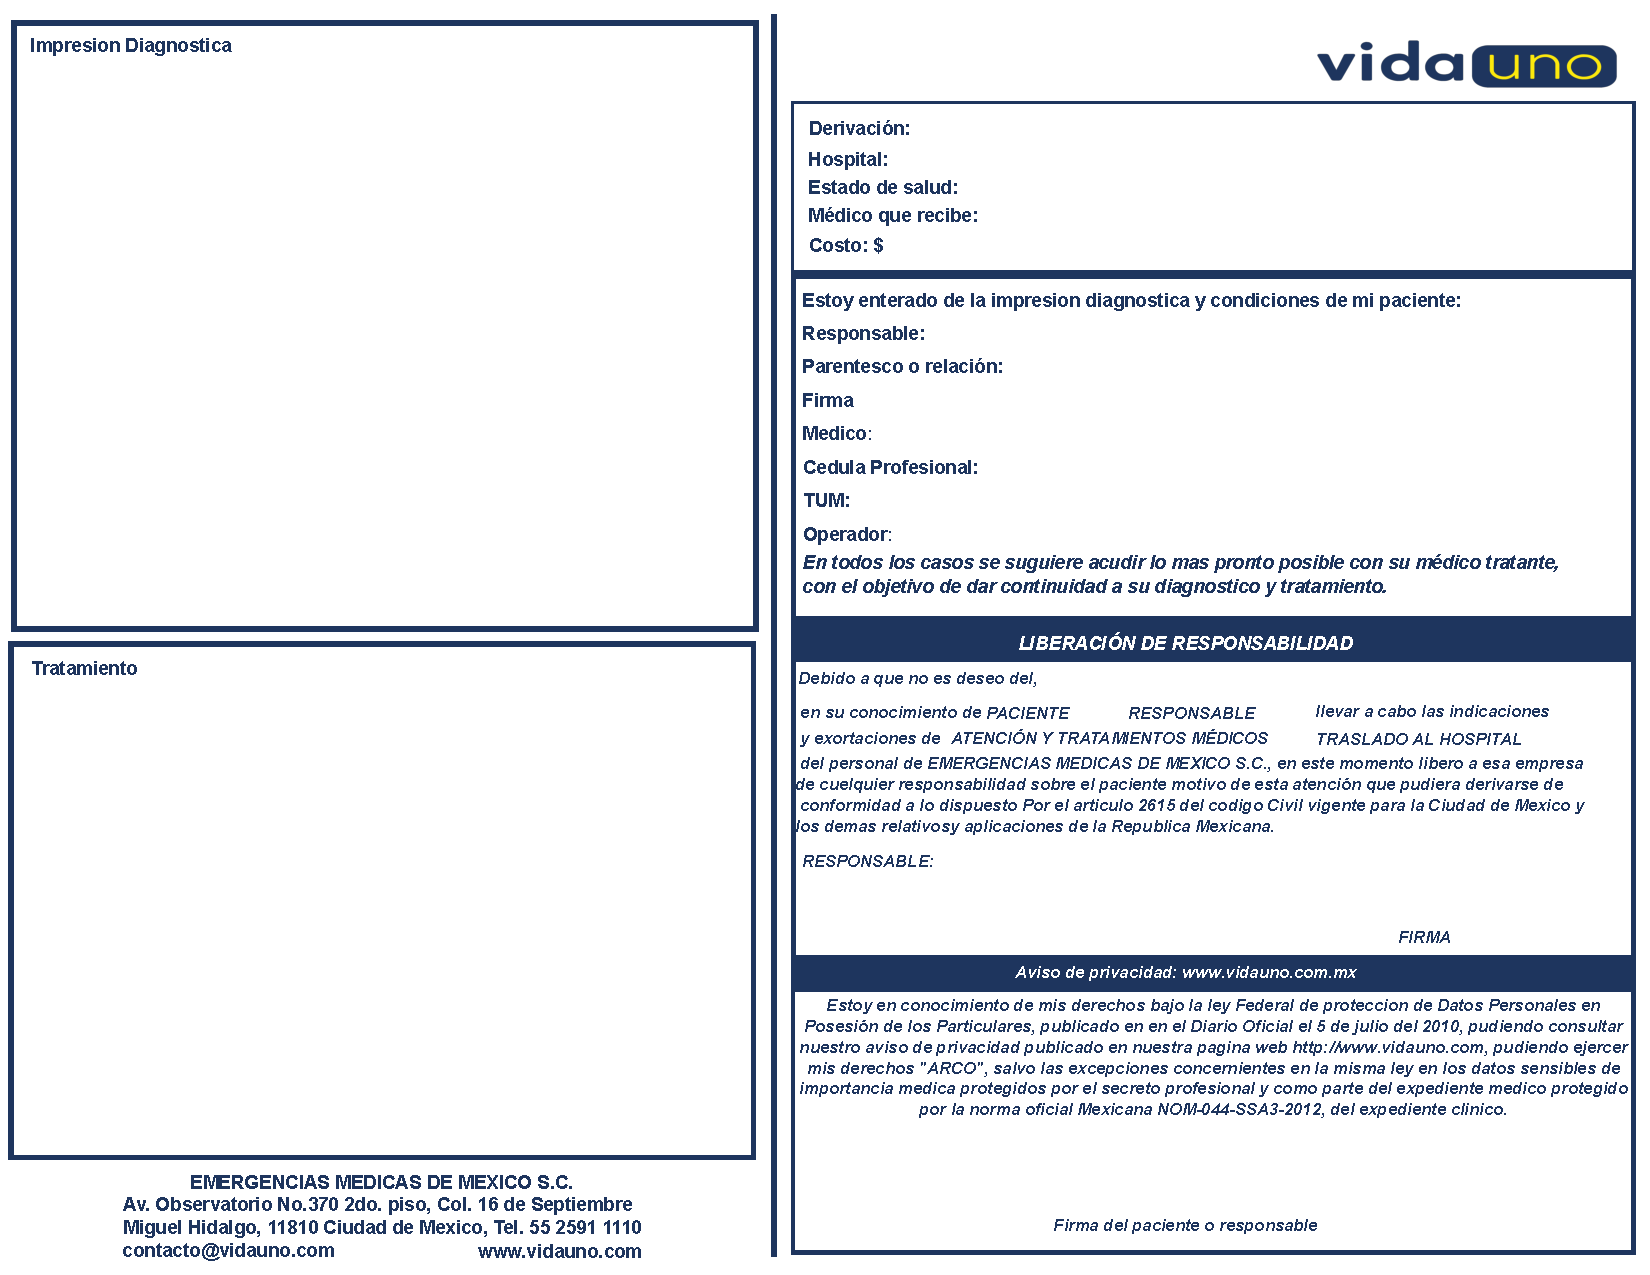
\includegraphics[width=\unitlength,page=1]{paperless_template_page_2}}%

    \put(0.42638971,0.73960084){\color[rgb]{0,0,0}\makebox(0,0)[lt]{\lineheight{1.25}\smash{\begin{tabular}[t]{l}\fontfamily{lmss}\selectfont 11\end{tabular}}}}%
    \put(0.43014479,0.72364315){\color[rgb]{0,0,0}\makebox(0,0)[lt]{\lineheight{1.25}\smash{\begin{tabular}[t]{l}\fontfamily{lmss}\selectfont M011\end{tabular}}}}%
   	\put(0.33829987,0.69381105){\color[rgb]{0,0,0}\makebox(0,0)[lt]{\lineheight{1.25}\smash{\begin{tabular}[t]{l}\fontfamily{lmss}\selectfont NA\end{tabular}}}}%
    \put(0.39132267,0.67728521){\color[rgb]{0,0,0}\makebox(0,0)[lt]{\lineheight{1.25}\smash{\begin{tabular}[t]{l}\fontfamily{lmss}\selectfont NA\end{tabular}}}}%

    %Paciente
    \put(0.09655761,0.62796396){\color[rgb]{0,0,0}\makebox(0,0)[lt]{\lineheight{1.25}\smash{\begin{tabular}[t]{l}\fontfamily{lmss}\selectfont F55\end{tabular}}}}%
    \put(0.20912356,0.62853648){\color[rgb]{0.11764706,0.20784314,0.36862745}\makebox(0,0)[lt]{\lineheight{1.25}\smash{\begin{tabular}[t]{l}\fontfamily{lmss}\selectfont 5556782349\end{tabular}}}}%
    \put(0.3268484,0.62911649){\color[rgb]{0,0,0}\makebox(0,0)[lt]{\lineheight{1.25}\smash{\begin{tabular}[t]{l}\fontfamily{lmss}\selectfont Masculino\end{tabular}}}}%
    \put(0.42764439,0.62796396){\color[rgb]{0,0,0}\makebox(0,0)[lt]{\lineheight{1.25}\smash{\begin{tabular}[t]{l}\fontfamily{lmss}\selectfont 15\end{tabular}}}}%
    \put(0.12766308,0.61324599){\color[rgb]{0,0,0}\makebox(0,0)[lt]{\lineheight{1.25}\smash{\begin{tabular}[t]{l}\fontfamily{lmss}\selectfont SHEEE Sanchez Jaime\end{tabular}}}}%
    \put(0.02575936,0.58169366){\color[rgb]{0,0,0}\makebox(0,0)[lt]{\lineheight{1.25}\smash{\begin{tabular}[t]{l}\fontfamily{lmss}\selectfont NA\end{tabular}}}}%


    %Paciente desconocido
    \put(0.01413581,0.52820903){\color[rgb]{0,0,0}\makebox(0,0)[lt]{\lineheight{1.25}\smash{\begin{tabular}[t]{l}\fontfamily{lmss}\selectfont \end{tabular}}}}%
    \put(0.01376544,0.48794778){\color[rgb]{0,0,0}\makebox(0,0)[lt]{\lineheight{1.25}\smash{\begin{tabular}[t]{l}\fontfamily{lmss}\selectfont  NA\end{tabular}}}}%
    \put(0.01355075,0.45100148){\color[rgb]{0,0,0}\makebox(0,0)[lt]{\lineheight{1.25}\smash{\begin{tabular}[t]{l}\fontfamily{lmss}\selectfont NA\end{tabular}}}}%
    \put(0.11853319,0.43470284){\color[rgb]{0,0,0}\makebox(0,0)[lt]{\lineheight{1.25}\smash{\begin{tabular}[t]{l}\fontfamily{lmss}\selectfont NA\end{tabular}}}}%

    %Padecimiento
    \put(0.02265882,0.24439213){\color[rgb]{0,0,0}\makebox(0,0)[lt]{\lineheight{1.25}\smash{\begin{tabular}[t]{l}\fontfamily{lmss}\selectfont NA\end{tabular}}}}%

    %Antecedentes
    %Diabetes
    \put(0.01071591,0.15522432){\color[rgb]{0.11764706,0.20784314,0.36862745}\makebox(0,0)[lt]{\lineheight{1.25}\smash{\begin{tabular}[t]{l}Diabetes mellitus\end{tabular}}}}%
    \put(0.1162418,0.15515692){\color[rgb]{0.11764706,0.20784314,0.36862745}\makebox(0,0)[lt]{\lineheight{1.25}\smash{\begin{tabular}[t]{l}- Si1 -\end{tabular}}}}%  
    \put(0.14649555,0.15522432){\color[rgb]{0.11764706,0.20784314,0.36862745}\makebox(0,0)[lt]{\lineheight{1.25}\smash{\begin{tabular}[t]{l}Diabetes melitus tipode evolucion y terapeutica actual\end{tabular}}}}%
    %Hipertension
    \put(0.01068221,0.14181276){\color[rgb]{0.11764706,0.20784314,0.36862745}\makebox(0,0)[lt]{\lineheight{1.25}\smash{\begin{tabular}[t]{l}Hipertension arterial\end{tabular}}}}%
    \put(0.1162418,0.14066955){\color[rgb]{0.11764706,0.20784314,0.36862745}\makebox(0,0)[lt]{\lineheight{1.25}\smash{\begin{tabular}[t]{l}- Si2 -\end{tabular}}}}%
    \put(0.14662476,0.14188016){\color[rgb]{0.11764706,0.20784314,0.36862745}\makebox(0,0)[lt]{\lineheight{1.25}\smash{\begin{tabular}[t]{l}hipertension arterial tipode evolucion y terapeutica actual\end{tabular}}}}%

  \end{picture}
\endgroup%
\end{figure}


\end{document}
